\documentclass[lettersize,journal]{IEEEtran}

% ====== 基础包 ======
\usepackage{amsmath,amsfonts,amssymb}
\usepackage{algorithm}
\usepackage{algorithmic}
\usepackage{array}
\usepackage[caption=false,font=normalsize,labelfont=sf,textfont=sf]{subfig}
\usepackage{textcomp}
\usepackage{stfloats}
\usepackage{url}
\usepackage{graphicx}
\usepackage{cite}
\usepackage{balance}

% ====== 表格与颜色 ======
\usepackage{booktabs}
\usepackage{multirow}
\usepackage{colortbl}
\usepackage{xcolor}
\usepackage{makecell}
\usepackage{amssymb}
\usepackage[most]{tcolorbox}

% ====== 中文支持（xelatex + xeCJK） ======
\usepackage{xeCJK}
\setCJKmainfont[BoldFont=SimHei,ItalicFont=KaiTi]{SimSun}
\setCJKsansfont{Microsoft YaHei}
\setCJKmonofont{FangSong}

% ====== 图片路径 ======
\graphicspath{{figures/}}

% ====== 颜色定义 ======
\definecolor{oursrow}{RGB}{228,238,255}
\definecolor{greenrow}{RGB}{228,245,228}
\definecolor{orangerow}{RGB}{255,240,225}
\definecolor{purplerow}{RGB}{240,230,250}
\definecolor{grayrow}{RGB}{245,245,245}
\definecolor{promptbg}{RGB}{242,247,253}
\definecolor{promptborder}{RGB}{70,130,180}

\newtcolorbox{promptbox}{
 colback=promptbg,
 colframe=promptborder,
 boxrule=0.5pt,
 arc=1mm,
 left=4pt,
 right=4pt,
 top=4pt,
 bottom=4pt,
 breakable,
 enhanced}

% ====== 自定义命令 ======
\newcommand{\best}[1]{\textbf{#1}}
\newcommand{\na}{\text{---}}
\newcommand{\posim}{\textsc{Posim}}

\hyphenation{op-tical net-works semi-conduc-tor IEEE-Xplore}

% ============================================================
\begin{document}
\raggedbottom

\title{POSIM：基于元认知智能体的通用社交媒体舆情仿真框架}

\author{作者（）%
\thanks{通讯作者信息（待补充）。}}

\markboth{IEEE}%
{POSIM：基于元认知智能体的通用社交媒体舆情仿真框架}

\maketitle

% ============================================================
% 摘要
% ============================================================
\begin{abstract}
社交媒体上的舆情事件可在数小时内引发大规模群体参与，理解并预判其演化过程对社会治理与危机应对具有重要价值。然而，现有仿真方法面临认知建模粗粒度、时间动力学失真和验证体系不完整三重挑战，难以忠实再现真实舆情的复杂动态。本文提出通用社交媒体舆情仿真框架POSIM（Public Opinion Simulator），将大语言模型嵌入EBDI（融合情感的信念-欲望-意图）分层认知框架，构建具有显式认知状态和可追溯推理链的元认知智能体。在仿真环境层面，框架采用霍克斯自激点过程统一建模外生事件冲击与内生用户交互，结合推荐算法与热搜榜单模拟，实现分钟级粒度的长周期高保真仿真。进一步地，框架建立了从微观机制校准到宏观涌现校准再到统计一致性校准的三层递进验证体系。在三个大规模真实微博舆情事件数据集上的实验表明，POSIM在行为分布、内容特征和网络拓扑三个层面均优于基线方法，且能自发涌现出情绪极化、无标度拓扑和信息级联幂律等与社会科学理论一致的宏观现象。此外，认知引导和反事实策略干预实验展示了框架在因果推理和舆情治理策略评估方面的应用价值——仿真中首次定量观察到共情悖论效应，并为危机公关策略的优选提供了实证依据。
\end{abstract}

\begin{IEEEkeywords}
社交媒体仿真，舆情分析，大语言模型，智能体认知架构，霍克斯过程
\end{IEEEkeywords}


% ============================================================
% 第1节 引言
% ============================================================
\section{引言}

社交媒体已成为公共舆论形成与传播的核心场域。在社交媒体平台上，一则突发事件可在数小时内引发数百万用户的参与讨论，形成复杂的群体情绪动态和信息级联效应~\cite{goldstein_structure_2012}。理解和预判舆情演化规律对社会治理、危机应对和公共政策制定具有重要的现实意义。然而，真实世界的社会实验面临伦理约束、不可重复性和变量不可控等根本性困难，使得基于计算机仿真的实验方法成为兼具科学严谨性和实践可操作性的研究路径~\cite{bonabeau_agent-based_2002}。

构建高保真的社交媒体舆情仿真系统面临三重核心挑战。第一，\textbf{认知建模挑战}：社交用户的行为决策充满非理性因素，受情绪驱动、认知偏差和社交影响等多重因素交互作用~\cite{kramer_experimental_2014}，如何使仿真智能体基于信念、情感和动机进行类人的非理性决策，而非作为简单的规则执行器或黑箱文本生成器，是实现微观行为保真度的前提。第二，\textbf{时间动力学挑战}：真实舆情事件中用户互动发生在分钟甚至秒级时间尺度——一条爆炸性新闻可在数分钟内引发数千条转发，而在事件间歇期活跃度则大幅回落——这种高度不均匀的时间分布对仿真的时间分辨率和计算效率提出了双重要求~\cite{zhao_seismic_2015}。第三，\textbf{验证闭环挑战}：仿真系统的可信度依赖于系统性的多层次验证，既需要校验微观决策机制的合理性，又需要验证宏观涌现现象的一致性，还需要与真实数据进行统计层面的定量比对~\cite{mcculloch_calibrating_2022}。

表~\ref{tab:comparison}对比了POSIM与现有代表性舆情仿真平台在关键能力维度上的差异。POSIM是首个同时具备认知机制建模、分钟级时间精度、真实数据评估、多策略推演支持和可扩展性的通用舆情仿真框架。

\begin{table}[!t]
\centering
\caption{POSIM与现有舆情仿真平台的能力对比}
\label{tab:comparison}
\renewcommand{\arraystretch}{1.0}
\resizebox{\columnwidth}{!}{%
\begin{tabular}{@{}lcccccc@{}}
\toprule
\textbf{平台} & \makecell{\textbf{认知}\\\textbf{机制}} & \makecell{\textbf{时间}\\\textbf{精度}} & \makecell{\textbf{真实数据}\\\textbf{验证}} & \makecell{\textbf{策略}\\\textbf{评估}} & \makecell{\textbf{可扩}\\\textbf{展性}} & \makecell{\textbf{多类}\\\textbf{智能体}} \\
\midrule
HiSim & $\times$ & $\star\star$ & $\checkmark$ & $\times$ & $\star\star$ & $\checkmark$ \\
LMAgent & $\times$ & $\star\star$ & $\checkmark$ & $\times$ & $\star\star$ & $\checkmark$ \\
SPARK & $\times$ & $\star\star$ & $\times$ & $\times$ & $\star\star$ & $\checkmark$ \\
S3 & $\times$ & $\star\star\star$ & $\checkmark$ & $\times$ & $\star\star\star$ & $\times$ \\
FDE-LLM & $\times$ & $\star\star$ & $\checkmark$ & $\times$ & $\star\star$ & $\checkmark$ \\
TrendSim & $\times$ & $\star\star\star\star$ & $\times$ & $\times$ & $\star\star\star$ & $\checkmark$ \\
OASIS & $\times$ & $\star\star\star\star$ & $\times$ & $\times$ & $\star\star\star\star$ & $\times$ \\
GA-S3 & $\times$ & $\star\star\star$ & $\checkmark$ & $\times$ & $\star\star$ & $\checkmark$ \\
\rowcolor{oursrow}
\textbf{POSIM (Ours)} & $\checkmark$ & $\star\star\star\star\star$ & $\checkmark$ & $\checkmark$ & $\star\star\star\star\star$ & $\checkmark$ \\
\bottomrule
\end{tabular}%
}
\vspace{2pt}
{\scriptsize \textit{注：} $\star$数量表示能力等级（1--5）。$\checkmark$ = 支持，$\times$ = 不支持。认知机制指显式BDI建模；时间精度指最细时间粒度与动态激活；策略评估指反事实干预支持。}
\end{table}

基于智能体的建模（ABM）方法因其天然适配社会系统自下而上涌现特性的优势，在舆情仿真中获得了广泛应用~\cite{macal_tutorial_2010}。经典的观点动态模型通过预定义的数值型交互规则刻画了个体观点在社交影响下的收敛、分裂和极化过程~\cite{castellano_statistical_2009}。然而，规则驱动的智能体无法生成真实的文本内容，仿真输出停留在数值层面，且固定规则难以覆盖人类认知决策的复杂性。近年来，大语言模型（LLM）的突破为社会仿真注入了新的可能性~\cite{wang_survey_2024}。以生成式智能体~\cite{park_generative_2023}为代表的研究证明了LLM驱动的智能体具备涌现复杂社会行为的潜力，后续工作进一步探索了LLM智能体在舆情仿真中的应用~\cite{gao_s3_2023,chuang_simulating_2024}。然而，多数现有工作将LLM作为端到端的行为映射器——直接从环境输入映射到行为输出——缺乏显式的中间认知状态建模，决策过程不可解释、不可追溯，且长周期仿真中智能体的人格一致性难以保证。

为应对上述挑战，本文提出社交媒体舆情仿真框架POSIM（\textbf{P}ublic \textbf{O}pinion \textbf{Sim}ulator）。该框架的核心思想是将LLM作为认知推理引擎嵌入基于EBDI（Emotion-augmented Belief-Desire-Intention）的分层认知架构，构建具备显式认知状态和可追溯推理链的元认知智能体。在仿真环境层面，框架采用霍克斯自激点过程建模群体活跃强度的时间动力学，并辅以多维度推荐算法和热搜榜单模拟，实现分钟级粒度的长周期高保真仿真。在验证层面，框架提出从微观机制校准到宏观涌现校准再到统计一致性校准的三层递进验证方法论。本文的主要贡献概括如下：

（1）提出元认知智能体架构，将LLM引入EBDI分层认知框架，构建了从感知、信念、欲望、意图到行为的完整认知链路。该架构通过层次化信念体系实现认知状态的显式建模与动态更新，通过多级思维链的意图规划实现可解释的行为生成，使每一步决策均可追溯至具体的认知状态变化。

（2）设计时间-事件混合驱动仿真环境，基于霍克斯自激点过程将外生舆情事件与内生用户交互统一纳入连续时间建模框架，使仿真的时间动态特性由数据驱动的点过程参数控制，而非依赖人工设定的固定时间步长。

（3）在三个大规模真实微博舆情事件数据集上进行了系统性的三层验证，并通过认知引导实验和反事实策略干预实验展示了框架在因果推理和舆情治理策略评估方面的应用价值，为舆情治理策略的定量评估提供了完整的实验闭环。


% ============================================================
% 第2节 相关工作
% ============================================================
\section{相关工作}
\label{sec:related}

\subsection{舆情建模与仿真}

早期舆情研究多将信息传播视作类传染过程。Daley和Kendall~\cite{daley_stochastic_1965}提出的随机谣言传播模型将个体划分为无知者、传播者和免疫者三类状态，通过马尔可夫链刻画谣言的扩散与消亡。这一范式后被广泛扩展，引入复杂网络结构和情绪传染因素~\cite{kramer_experimental_2014}，分析网络拓扑对级联规模和持续时间的影响。
随着社交媒体数据的积累，研究逐渐转向时间过程建模。一类工作采用生命周期与系统动力学框架刻画话题热度的阶段性演化~\cite{liu_evolution_2024,kong_exploring_2020}；另一类则使用点过程建模事件序列——Zhao等人~\cite{zhao_seismic_2015}提出SEISMIC模型预测推文流行度，Rizoiu等人~\cite{rizoiu_expecting_2017}发展了HIP框架统一建模反馈，Zhang等人~\cite{zhang_opinion-aware_2023}进一步将观点因素融入多变量点过程。然而，这一脉络通常将个体视为同质节点，内部信念与情绪过程被折叠进模型参数，难以解释细粒度的心理机制。\posim{}保留霍克斯过程在时间动力学上的优势，同时显式引入元认知智能体，使舆情演化既由点过程驱动，又由可追溯的认知链路支撑。

\subsection{基于智能体的社会仿真}

基于智能体的建模（ABM）通过为大量异质个体指定局部规则并观察涌现行为，已成为社会系统研究的重要范式~\cite{bonabeau_agent-based_2002,macal_tutorial_2010}。在观点动力学领域，DeGroot~\cite{degroot_reaching_1974}的共识达成模型和Hegselmann-Krause~\cite{hegselmann_opinion_nodate}的有界置信模型奠定了理论基础，Castellano等人~\cite{castellano_statistical_2009}从统计物理视角系统综述了社会动力学模型。
舆情方向的ABM工作通常在社交网络上构造多类用户和媒体代理，通过意见交换规则研究极化与回音室现象~\cite{liu_agent-based_2024,banisch_agent_2012}。ODD协议~\cite{grimm_odd_2010}和参数标定方法~\cite{mcculloch_calibrating_2022}为ABM提供了可复现的建模与验证流程。然而，多数舆情ABM仍依赖手工规则或有限状态机，难以覆盖真实语境中的复杂情绪反应和语言表达；时间维度往往停留在离散轮次更新，难以刻画不均匀的分钟级互动节奏。\posim{}继承ABM在主体异质性和可控性方面的优势，同时通过EBDI+LLM让规则以自然语言形式落地，使智能体既能生成真实文本，又能在连续时间环境中运行。

\subsection{大语言模型驱动的社会仿真}

近年来，大语言模型（LLM）的突破为社会仿真注入了新的可能性。Wang等人~\cite{wang_survey_2024}系统综述了LLM自主智能体的研究进展，Zhou等人~\cite{zhou_agents_2023}和Yang等人~\cite{yang_auto-gpt_2023}分别提出了通用的LLM智能体框架。Park等人~\cite{park_generative_2023}的生成式智能体开创性地证明了LLM驱动的智能体具备涌现复杂社会行为的潜力，在虚拟小镇中展示了记忆、规划和多智能体互动能力。
面向社交媒体的研究迅速跟进。Gao等人~\cite{gao_s3_2023}构建了S3系统模拟社交网络中的信息传播；Chuang等人~\cite{chuang_simulating_2024}研究了LLM智能体网络中的观点动力学；Zhang等人~\cite{zhang_spark_2025}提出SPARK模拟立场与话题的共演化；TrendSim~\cite{zhang_trendsim_2025}关注热搜话题的投毒攻击仿真；OASIS~\cite{yang_oasis_2025}实现了百万级智能体的社交互动仿真。在舆情预测方面，Yao等人~\cite{yao_social_2025}将动力学方程与LLM智能体融合，Zhang等人~\cite{zhang_llm-aidsim_2025}和Hu等人~\cite{hu_llm-enhanced_2024}探索了LLM增强的影响力扩散仿真，Mou等人~\cite{mou_unveiling_2024}研究了大规模社会运动仿真，Liu等人~\cite{liu_lmagent_2026}提出了多模态智能体社会框架。
尽管上述工作展示了LLM在内容生成和常识推理上的优势，但在认知建模、环境机制和验证闭环上仍存在不足：多数方法将LLM作为端到端策略函数，缺乏显式的信念/欲望/情绪状态表征；时间机制多为轮次驱动或脚本控制，较少引入点过程等数据驱动的连续时间模型；评估往往依赖少量宏观指标或案例分析，缺乏系统性的多层次验证。\posim{}通过EBDI分层认知架构赋予智能体可更新的内部状态，使用霍克斯过程加推荐与热搜机制构建贴近真实平台的环境，并设计从微观行为到宏观现象再到统计一致性的三层递进验证体系。
% ============================================================
% 第3节 方法（占位，后续步骤填充）
% ============================================================
\section{POSIM框架}
\label{sec:method}

本节详细介绍POSIM框架的三个核心组件：元认知智能体架构（第\ref{subsec:agent}节）、仿真环境（第\ref{subsec:env}节）和策略推演框架（第\ref{subsec:strategy}节）。图~\ref{fig:framework}展示了框架的整体架构。

% --- 框架总图占位 ---
\begin{figure*}[!t]
\centering

\includegraphics[width=0.75\textwidth]{framework_overview.pdf}
\caption{POSIM框架总体架构。左侧为元认知智能体架构，包含信念、欲望和意图三个认知子系统；中间为仿真环境，包含霍克斯点过程驱动的时间引擎、虚拟社交媒体平台；右侧为策略推演框架。}
\label{fig:framework}
\end{figure*}

% \subsection{问题定义}

% 社交媒体舆情仿真的目标是：给定一组初始用户群体$\mathcal{U}$、事件背景$\mathcal{B}$及外部事件序列$\mathcal{E} = \{e_1, e_2, \ldots, e_K\}$，在虚拟社交媒体平台上模拟用户群体在舆情事件中的行为演化过程$\{A_t\}_{t=0}^{T}$，使得仿真产生的宏观统计特征（行为分布、情感动态、网络拓扑等）与真实舆情数据具有统计一致性，同时智能体的微观决策过程具备认知可解释性。

\subsection{元认知智能体架构}
\label{subsec:agent}

传统的反应式智能体遵循简单的感知--行动范式，仅作为无状态的行为生成器，无法捕捉人类决策中涉及信念修正、动机权衡和策略选择的复杂认知机制。考虑到社交媒体用户的行为决策受情绪驱动、认知偏差和社交影响等多重非理性因素的交互作用，我们提出融合情感因素的元认知智能体架构。元认知体现在两个层面：其一，智能体具有显式的自我认知状态，每一步决策均基于可观测的认知状态变化；其二，智能体的认知过程本身是可审计的多阶段推理链，而非单次黑箱调用。认知流程形式化为：
\begin{multline}
\text{Perception}(P_t) \!\to\! \text{Belief}(B_t) \!\to\! \text{Desire}(D_t) \\
\to\, \text{Intention}(I_t) \!\to\! \text{Action}(A_t)
\end{multline}

该架构以LLM为认知推理引擎，包含信念子系统、欲望子系统和意图子系统三个核心模块。三个子系统在每个决策周期内依次运行，各自接收上游输出作为输入，形成从环境感知到行为输出的完整且可追溯的认知链路。

\subsubsection{信念子系统}

信念是智能体对外部世界和自身状态的动态认知表征，构成一切决策推理的基础。社会心理学研究表明，个体的不同认知层次具有不同的稳定性——核心人格特质在短期内高度稳定，而对特定事件的观点和即时情绪则随信息输入快速变化。基于这一认知分层特性，我们设计了层次化的信念体系$B = \langle B^{id}, B^{psy}, B^{evt}, B^{emo} \rangle$，四类信念按认知修正难度从高到低排列。

\textbf{角色身份信念}$B^{id}$表征智能体的固有基础认知，包括人口学属性（性别、地域）、社交属性（粉丝规模、认证类型）和身份属性（职业、兴趣标签）等，在仿真周期内保持恒定。例如，``我是一名拥有10万粉丝的微博认证博主，关注领域为社会时事''。初始化时，从真实社交媒体平台采集用户的基础信息及历史发布内容，利用LLM进行结构化推断，以第一人称自述的自然语言形式生成角色身份描述。该信念在仿真过程中不会更新，作为智能体人格一致性的锚定层。

\textbf{心理认知信念}$B^{psy}$表征智能体在舆情参与中的深层心理特征与认知倾向。社会心理学研究表明，网民在面对网络事件时表现出从众、成见、冲动、偏执等典型心理现象。基于对多起真实舆情事件中用户行为模式的分析，我们将网民心理特征归纳为以下典型模式：自我实现型（追求社会认同与自我价值实现）、猎奇探究型（对新奇事件保持高度关注）、减压宣泄型（将网络空间视为情绪释放渠道）、仇官仇富型（对权力与财富持有负面预设）、跟风从众型（倾向于追随主流意见）等。心理认知信念以结构化文本列表形式存储，每条信念为一个具体的认知倾向描述，如``主流媒体未报道的往往才是真相''``富人的财富来源存疑''等。初始化时，基于采集的真实用户历史内容，通过LLM从预定义的心理特征池进行个性化采样与适配。心理认知信念在仿真过程中保持高度稳定，反映了深层心理特质的抗变性。

\textbf{事件观点信念}$B^{evt}$表征智能体对特定舆情事件中各参与主体的事实认知、背景理解和观点立场。与前两类信念不同，事件观点信念随舆情发展动态演化——新信息的摄入、他人观点的影响和事件进展均可能导致观点的修正或强化。每条事件观点采用结构化四元组表示：$\langle t, \text{subject}, \text{opinion}, \text{reason} \rangle$，其中$t$为观点形成时间，subject为评价主体（如涉事人物、机构等），opinion为当前观点立场，reason为支持该观点的理由。初始化时，基于用户在事件爆发前的历史发布内容，通过LLM驱动的结构化深度访谈机制（如提问``对于涉事主体X，你当前的观点是什么？''）提取用户对各参与主体的初始观点倾向。

\textbf{情绪激发信念}$B^{emo}$基于认知行为理论中的ABC模型，强调认知评价对情绪反应和后续行为的中介作用。情绪周期现象是后真相时代网络舆情的显著特征——事件初期的情绪爆发、中期的情绪传染与极化、后期的情绪衰减构成了完整的情绪动力学过程。为建模这一过程，我们采用Ekman的六维基本情感分类框架，将情绪状态表征为连续向量$\mathbf{e} = [e_{hap}, e_{sad}, e_{ang}, e_{fear}, e_{sur}, e_{dis}]^\top \in [0,1]^6$，分别对应快乐、悲伤、愤怒、恐惧、惊讶和厌恶六种基本情绪。情绪状态的更新受三个机制驱动：（1）\textbf{时间衰减}——参照心理学中情绪的自然消退规律，情绪强度随时间按指数衰减：$\mathbf{e}_i(t) = \mathbf{e}_i(t_0) \cdot e^{-\lambda_e(t-t_0)}$，其中$\lambda_e$为衰减系数；（2）\textbf{内容刺激}——智能体浏览的推荐内容中蕴含的情感色彩对其情绪产生增量影响：$\mathbf{e}_i \leftarrow \mathbf{e}_i + \eta \cdot \mathbf{s}_{content}$，其中$\mathbf{s}_{content}$为内容的情感向量，$\eta$为影响系数；（3）\textbf{社交传染}——智能体的情绪受其社交邻居的情绪状态影响：$\mathbf{e}_i \leftarrow (1-\rho) \cdot \mathbf{e}_i + \rho \cdot \bar{\mathbf{e}}_{neighbor}$，其中$\bar{\mathbf{e}}_{neighbor}$为邻居情绪均值，$\rho$为传染强度系数。

\textbf{信念更新机制。}信念更新基于双通道信息输入：外部环境感知$P_t$与历史行为记忆$M_t$。历史记忆采用流式记忆库存储，检索时使用同时兼顾时间衰减与语义相似度的加权打分函数：
\begin{equation}
R(m, t) = \alpha_{\mathrm{rec}} e^{-\gamma(t - t_m)} + (1-\alpha_{\mathrm{rec}})\,\text{sim}(q, m),
\label{eq:mmr}
\end{equation}
其中$\text{sim}(\cdot,\cdot)$为基于预训练编码器的余弦相似度，$\alpha_{\mathrm{rec}}\in[0,1]$控制"近因性"与"相关性"之间的权衡。在推理过程中，我们通过提示词显式引入确认偏差、锚定效应、情绪优先推理和简单归因倾向等认知偏差，以模拟真实人类认知中的系统性偏差。信念更新的整体形式为：
\begin{equation}
B_{t+1} = f_{\text{LLM}}(B_t, P_t, M_t, \Phi)
\label{eq:belief_update}
\end{equation}
其中$\Phi$为嵌入提示词中的认知偏差引导。更新主要作用于$B^{evt}$和$B^{emo}$两个快速变化层，同时以较小步长缓慢调整$B^{psy}$中的心理认知信念，使其在长期尺度上随历史经验发生渐进演化；$B^{id}$作为身份锚点在仿真过程中保持不变。

\subsubsection{欲望子系统}

欲望子系统承担动机生成器的角色——将信念状态转化为行为动机。社交媒体用户的参与动机高度多样化且因人而异，难以用固定规则覆盖，因此我们利用LLM的常识推理能力自动推断当前欲望集合。欲望集合采用带权重的多目标列表表示：
\begin{equation}
D_t = \{(d_1, w_1), (d_2, w_2), \ldots, (d_n, w_n)\}, \quad w_i \in [0, 1]
\end{equation}

基于使用与满足理论，我们定义了七类典型欲望：情绪宣泄、娱乐消遣、自我表达、社交认同、社交连接、正义倡导和信息获取。欲望列表为意图子系统的行为规划提供动机约束——例如，当情绪宣泄欲望强度最高时，智能体更倾向于选择短评论和激烈的情感表达。欲望生成函数形式化为$D_t = g_{\text{LLM}}(B_{t+1}, P_t)$。

\subsubsection{意图子系统}

意图子系统作为认知链路的最终决策环节，承担层级行为规划器的角色。\posim{}将社交媒体上的原子行为抽象为点赞、直接转发、转发带评论、评论以及原创博文等几类交互形式，而不再依赖精确的字数阈值来区分“长短”内容。与传统的单步行为生成不同，意图子系统采用多级思维链机制，将行为决策分解为三个递进的推理层级：

\textbf{第一级——行为类别与目标对象选择：}LLM根据信念状态和欲望强度分布，从七种原子操作中选择行为类别，并确定互动的目标对象。该层级决定做什么和对谁做。例如，当情绪宣泄欲望强度最高且愤怒情绪占主导时，智能体更倾向于选择短评论或转发带评论等能快速表达情绪的行为类型。

\textbf{第二级——表达策略规划：}在四个正交维度上规划表达策略——（a）\textit{情绪维度}：主导情绪类型（愤怒、厌恶、焦虑、悲伤、兴奋、中性等）与强度等级（低/中/高/极端）；（b）\textit{立场维度}：对目标主体的支持/反对/中立立场及其强度；（c）\textit{风格维度}：理性分析、讽刺调侃、情绪攻击、共情理解、质疑求证等表达风格；（d）\textit{叙事维度}：事实罗列、标签化、行动呼吁、权威引用、阴谋论等叙事策略。该层级决定以何种方式表达。

\textbf{第三级——内容生成：}基于前两级决策的约束，生成符合角色特征的具体文本内容，包括正文、话题标签和@提及。该层级决定具体说什么。例如，当第二级规划为高强度愤怒、反对立场、讽刺风格和标签化叙事时，生成的内容将呈现激烈的情绪表达、明确的反对态度和讽刺性的修辞手法。

这种三级分解设计具有两方面优势：其一，为内容生成提供了显式的策略约束，避免LLM在无引导下倾向于生成平均化的温和文本；其二，每一级的决策结果均被记录，使得行为的生成过程完全可追溯——研究者可从表达策略中分析为何智能体选择了特定的情绪基调或叙事手法。整体意图生成过程形式化为$I_t = h_{\text{LLM}}(B_{t+1}, D_t, P_t)$，输出行为序列$I_t = \{(a_j, o_j, s_j, c_j)\}_{j=1}^{m}$，其中$a_j$为行为类型，$o_j$为目标对象，$s_j = (\text{emotion}, \text{stance}, \text{style}, \text{narrative})$为表达策略向量，$c_j$为生成内容。单个智能体在每个决策周期内可生成$m \geq 0$个行为，$m$的值由LLM根据事件热度、情绪强度和用户活跃倾向自主决定。

\subsubsection{异质性智能体}

真实舆情演化涉及多类主体的复杂交互。基于元认知架构，我们定义了四种异质性智能体类型，它们共享同一套EBDI认知管线，但在角色约束和行为偏好上存在系统性差异：\textbf{普通网民}构成舆情参与的绝对主体，行为受个人信念和情绪主导，语言风格口语化，偏好短评论和点赞等轻量级交互；\textbf{意见领袖}具有较大影响力，决策更注重影响力维护和独立观点输出，活跃度最高；\textbf{媒体智能体}注重信息的时效性和权威性，以长博文为主，情绪表达克制；\textbf{政府智能体}代表官方立场，以高原创比例的长博文为核心行为形式。差异化行为通过角色特化提示词和行为参数差异化两个机制实现。

附录图~\ref{fig:cognitive_example}展示了一个普通网民智能体在单个仿真步内的完整认知链路实例，涵盖从环境感知到信念更新、欲望生成、意图规划与行为执行的全过程，清晰展示了EBDI架构中各认知模块的输入-输出关系和信息流动。

\subsection{仿真环境}
\label{subsec:env}

仿真环境是智能体感知和交互的虚拟社交媒体平台，其设计目标是在保持计算可行性的前提下忠实再现真实社交平台的信息流动机制和时间动力学特性。

\subsubsection{时间-事件混合驱动内核}

真实舆情事件中用户互动发生在分钟级时间尺度——一条爆炸性新闻可在数分钟内引发数千条转发，而在事件间歇期活跃度则大幅回落。传统的固定时间步长激活模式无法适应这种时间尺度的剧烈波动。为此，我们采用霍克斯自激点过程作为群体活跃强度的生成模型。霍克斯过程的核心特性在于历史事件提升未来事件的发生概率，与舆情中热点事件激发参与、参与催生更多参与的正反馈机制高度吻合。如图~\ref{fig:framework}右上角所示，条件强度函数定义为：
\begin{equation}
\lambda(t) = \mu + \sum_{t_i < t} \phi(t - t_i)
\label{eq:hawkes}
\end{equation}
其中$\mu$为基础活跃率，$\phi(t) = \alpha e^{-\beta t}$为指数衰减的激励核函数。激励项包含两类来源：（1）\textbf{外部事件刺激}$\phi_{ext}$——外生舆情事件以较大的激励强度$\alpha_{ext}$和较慢的衰减$\beta_{ext}$注入活跃度脉冲；（2）\textbf{内部活跃刺激}$\phi_{int}$——用户行为本身以较弱的激励$\alpha_{int} \ll \alpha_{ext}$和较快的衰减$\beta_{int} \gg \beta_{ext}$产生二阶正反馈。为模拟社交媒体用户在工作日与夜间、工作日与周末之间的系统性活跃差异，我们进一步引入昼夜节律调制函数$\lambda_{adj}(t) = \lambda(t) \cdot [(1 - s) + s \cdot \text{circ}(h(t))]$：当$\text{circ}(h(t))$在白天取高值、夜间取低值时，相同的外生事件在不同时段会诱发不同水平的集体响应，从而在无需额外脚本控制的情况下自然生成“白天高峰、夜间低谷”的日周期模式。

在每个时间步$\Delta t$内，系统根据调制后的强度采样当步需要激活的智能体数量：
\begin{equation}
N_t \sim \text{Poisson}\!\bigl(\lambda_{adj}(t)\, N_{\text{scale}}\bigr),
\end{equation}
其中$N_{\text{scale}}$是将连续强度映射为期望激活人数的缩放系数。被激活的智能体通过加权采样确定，采样概率与其活跃度权重$A(u_i)$成正比，
\begin{equation}
P(u_i \text{ activated}) \propto A(u_i),
\end{equation}
其中$A(u_i)$综合考虑用户长期发帖频率与社交影响力，并在$[0,1]$区间内进行归一化。

\subsubsection{社交媒体推荐机制}

推荐算法是信息传播的守门人，决定了用户看到什么内容，进而影响其信念更新和行为决策。基于社交媒体平台内容推荐算法的通用思想，对于用户$u$和候选内容$p$，我们设计了由三个维度加权组合得到的曝光得分函数：
\begin{equation}
S_{exp}(u, p) = \alpha \cdot H(u, p) + \beta \cdot P(p) + \gamma \cdot R(p)
\label{eq:recommend}
\end{equation}
其中$H(u, p) = \cos(\mathbf{e}_u, \mathbf{e}_p)$为同质性得分，基于用户画像嵌入与内容嵌入的余弦相似度，模拟信息茧房效应——用户更容易看到与自身兴趣和立场相近的内容；$P(p)$为基于点赞、转发、评论等多维互动信号归一化得到的热度得分，用于刻画内容在全局范围内的受关注程度；$R(p) = e^{-\mu_r(t - t_p)}$为新鲜度得分，保证新内容获得曝光优势。语义嵌入采用BGE-small-zh-v1.5模型编码，并实施语义去重以避免信息冗余。

为平衡个性化推荐与信息多样性，候选内容按来源分为关注用户和非关注用户两个桶，按类型分为原创和转发两个桶，分桶独立排序后合并。系统保留$20\%$的探索位用于随机推荐用户未接触过的内容，以抑制过度的信息茧房效应。每轮仿真中，智能体获取不超过$K$条推荐结果（默认$K{=}10$），每条内容附带$N_c$条随机采样的评论（默认$N_c{=}5$），模拟用户浏览评论区的行为。此外，系统根据仿真中涌现的话题标签自动统计热度（综合提及次数、互动量和时间衰减），定期更新热搜排行榜，上榜话题作为额外的信息曝光渠道呈现给智能体，模拟真实平台中热搜对舆情注意力聚焦的放大效应。

\subsection{策略推演框架}
\label{subsec:strategy}

POSIM不仅是一个仿真器，更是一个支持策略评估的实验平台。为支持舆情治理策略的定量评估和反事实分析，框架构建了由\textbf{策略干预}、\textbf{策略推演}和\textbf{策略评估}三个模块组成的仿真循环闭环（图~\ref{fig:framework}右侧）。

\textbf{策略干预}是连接外部治理意图与仿真内部状态的统一接口层，采用事件队列的形式实现。每个干预事件以五元组$E = \langle t, \tau, s, c, \iota \rangle$表示，并提供三个粒度的接口化注入方式：（1）\textit{用户级干预}——针对特定智能体进行定点控制，如指定KOL在特定时间发布引导内容、修改目标用户的信念状态或行为约束；（2）\textit{事件级干预}——面向全体智能体的全局广播，如注入外部突发事件、发布官方通告或触发新闻报道；（3）\textit{平台级干预}——调整仿真环境的运行参数，如修改推荐算法权重、调整热搜榜单策略或设置内容过滤规则。三类干预通过标准化接口注入仿真系统，支持任意组合和时序编排。\textbf{策略推演}模块负责将设计好的干预方案转化为可执行的仿真实验。该模块由一组仿真回调器（Simulation Callbacks）组成，基于状态快照机制，系统支持从任意仿真时间步创建分支，对同一基线下的不同干预方案进行并行仿真推演。每个回调器独立管理一个仿真分支的生命周期——包括快照恢复、干预注入、仿真推进和结果输出——使得多种策略的对比实验可以在统一的实验条件下高效并行执行。\textbf{策略评估}模块与仿真引擎完全解耦，通过标准化数据接口读取仿真日志系统的输出，独立计算多层次评估指标。评估器的解耦设计支持用户根据具体研究需求灵活定义评估维度和指标体系——例如情绪极化指数、行为类型分布、话语对抗性等——而无需修改仿真引擎或智能体模块。日志系统完整记录每步仿真的智能体认知状态、行为决策和环境变量，为事后分析和可解释性追溯提供数据基础。上述三个模块构成策略干预$\to$策略推演$\to$策略评估的仿真循环，评估结果可反馈指导新一轮干预方案的设计与优化，支撑迭代式的策略探索与决策支持。

\textbf{LLM资源调度。}大规模仿真涉及大量LLM调用，框架通过统一的API资源池管理多个LLM端点，支持多模型混合驱动和按用途路由——信念更新、欲望生成和行为决策三个认知阶段可分别指定不同规模的模型，兼顾推理质量与成本效率。资源池实现了端点级并发控制（信号量机制）、轮询式负载均衡、故障自动检测与转移以及调用频率限制，确保在高并发场景下的稳定运行。为避免LLM产生同质化输出，系统对每次调用的采样参数进行随机扰动：Temperature扰动$T' = T + \epsilon_T$，$\epsilon_T \sim \mathcal{U}(-0.1, 0.1)$；Top-p扰动$p' = p + \epsilon_p$，$\epsilon_p \sim \mathcal{U}(-0.05, 0.05)$；并随机注入频率惩罚和存在惩罚参数以增加词汇和话题多样性。

\textbf{模块化架构。}POSIM采用高度解耦的模块化设计，智能体模块、环境模块和策略推演模块三大核心模块相互独立，通过标准化接口通信。全局仿真参数通过统一的配置文件管理，支持不同舆情事件的快速适配。这一设计支持独立替换和扩展——例如，可以在不修改环境模块的前提下引入新的智能体认知架构，或在不修改智能体模块的前提下替换推荐算法。


% ============================================================
% 第4节 实验（占位，后续步骤填充）
% ============================================================
\section{实验}
\label{sec:exp}

\subsection{实验设置}

\subsubsection{数据集}

实验基于从新浪微博平台采集的三个具有代表性的大型社会舆情事件数据集展开。\textbf{天价耳环事件}（LE）：2025年5月，演员黄杨钿甜成人礼照片中佩戴的绿色耳饰被网友指认为奢侈品牌耳环，引发公众对明星炫富与青少年价值观的争议；\textbf{武汉大学图书馆事件}（WL）：2025年7月，武汉大学图书馆管理纠纷引发校园治理与学生权益的广泛讨论；\textbf{西贝预制菜事件}（XF）：2025年9月，西贝莜面村预制菜争议引发公众对食品安全和消费者权益的持续关注。数据经过去重、低活跃用户过滤（事件期间发帖$<$2条）和无关内容清洗（广告、商业推广、不相关话题）后的描述性统计见表~\ref{tab:dataset}。仿真时间精度为10分钟/步。

\textbf{智能体信念初始化。}信念初始化直接决定了智能体的个性化程度。对于每个用户，基于其在仿真起始时间之前的历史发布内容，通过以下流程构建EBDI信念系统：（1）角色身份信念——将用户基础信息和历史内容摘要输入LLM，生成第一人称角色描述；（2）心理认知信念——从涵盖八类典型网民心理模式的特征池中，基于历史内容的语义匹配进行个性化采样；（3）事件观点信念——通过LLM驱动的结构化深度访谈提取对各涉事主体的初始观点；（4）初始情绪向量——基于近期发布内容的情感分析结果初始化六维情绪向量。

\begin{table}[!t]
\centering
\caption{三个舆情事件数据集的描述性统计}
\label{tab:dataset}
\renewcommand{\arraystretch}{1.0}
\resizebox{\columnwidth}{!}{%
\begin{tabular}{@{}lccccc@{}}
\toprule
\textbf{事件} & \textbf{用户数} & \textbf{博文数} & \textbf{时长} & \textbf{仿真步数} & \textbf{类型} \\
\midrule
天价耳环 (LE) & 1,530 & 34,218 & $\sim$46h & 276 & 社会争议 \\
武大图书馆 (WL) & 1,843 & 51,647 & $\sim$190h & 1,140 & 校园事件 \\
西贝预制菜 (XF) & 1,987 & 14,892 & $\sim$71h & 426 & 食品安全 \\
\bottomrule
\end{tabular}%
}
\end{table}

\subsubsection{验证框架}

仿真模型的可信度评估是社会仿真研究的核心挑战。本文的验证框架受仿真工程领域经典的V\&V（Verification and Validation）原则启发~\cite{sargent_verification_2013}。V\&V方法论起源于系统工程与国防仿真领域，其核心思想将模型评估分为两个互补维度：\textbf{验证}（Verification）回答``我们是否正确地构建了模型？''——即检验计算模型是否忠实实现了概念模型的设计意图；\textbf{确认}（Validation）回答``我们是否构建了正确的模型？''——即检验模型输出是否准确反映了目标系统的真实行为。基于这一原则，仿真系统的验证遵循三层递进框架：（1）\textbf{微观行为机制校准}（Verification）——验证智能体是否按照设计意图做出认知上可解释的决策；（2）\textbf{宏观现象涌现校准}（Emergence Validation）——验证微观机制能否涌现出符合社会科学理论预期的宏观现象；（3）\textbf{统计结果一致性校准}（Validation）——验证仿真输出是否在统计意义上准确再现真实舆情动态。三个层次构成从内部正确性（Verification）、涌现合理性到外部准确性（Validation）的完整验证链，系统覆盖了V\&V方法论的核心评估维度。

\subsubsection{对比方法}

微观验证设置四种决策方法：\textbf{Direct-Nothink}（轻量模型单次提示直接输出行为）、\textbf{Direct-Think}（较强模型单次提示直接输出）、\textbf{CoT}（单次调用内完成信念-欲望-行为的思维链串联）和\textbf{EBDI}（本文方法，三阶段独立模块多步推理）。统计校准设置三种对比基线：\textbf{Rule-based ABM}（预定义规则驱动的传统仿真）、\textbf{POSIM w/o EBDI}（移除认知架构，LLM单步决策）和\textbf{POSIM w/ CoT}（将EBDI替换为单次思维链推理）。

\subsection{微观行为机制验证}

微观验证旨在回答核心问题：EBDI元认知架构是否使智能体具备了类人的、在认知与行为上可解释的决策能力？智能体在微观层面的行为机制一致性——即其决策是否遵循可理解的认知逻辑、是否保持人格稳定性、是否具备对输入扰动的认知鲁棒性——决定了宏观涌现结果的可信度基础。

实验基于天价耳环事件，随机抽取$N=100$名用户作为智能体，每名智能体具备从真实数据中初始化的身份描述、心理认知信念与行为倾向。仿真共进行$T=12$轮，四种方法在相同的事件背景、用户池和轮次下运行，仅决策接口与是否保留中间认知状态不同，以保证对比的公平性。评估阶段使用Qwen2.5-14B-Instruct（temperature$=0.3$）作为LLM-as-Judge。三个评估维度的计算方式如下：（1）\textbf{认知行为链一致性}——将每个智能体在全部轮次的完整认知-行为记录提交评估LLM，从认知链完整性、情绪动态合理性、动机-行为对齐度和信息整合能力四个子维度进行0--5分等级评分；（2）\textbf{人格稳定性}——评估LLM基于行为轨迹反推智能体的身份描述和行为倾向，与初始设定计算相似度（0--1）；（3）\textbf{认知鲁棒性}——对输入进行语义等价扰动（博文顺序打乱、随机删减、加入无关博文），每条原始决策对应5次扰动重复，评估核心决策稳定性和认知锚定强度（0--1）。结果见表~\ref{tab:micro}。

\begin{table}[!t]
\centering
\caption{微观行为机制验证结果（均值$\pm$标准差）}
\label{tab:micro}
\renewcommand{\arraystretch}{1.0}
\resizebox{\columnwidth}{!}{%
\begin{tabular}{@{}lccc@{}}
\toprule
\textbf{方法} & \makecell{\textbf{认知行为链}\\\textbf{一致性} (0--5)\,$\uparrow$} & \makecell{\textbf{人格}\\\textbf{稳定性} (0--1)\,$\uparrow$} & \makecell{\textbf{认知}\\\textbf{鲁棒性} (0--1)\,$\uparrow$} \\
\midrule
Direct-Nothink & 1.47$\pm$0.50 & 0.478$\pm$0.263 & 0.629$\pm$0.240 \\
\rowcolor{grayrow}
Direct-Think & 1.75$\pm$0.43 & 0.448$\pm$0.269 & 0.603$\pm$0.299 \\
CoT & 3.09$\pm$0.29 & 0.516$\pm$0.272 & 0.541$\pm$0.356 \\
\rowcolor{greenrow}
\textbf{EBDI (Ours)} & \best{4.64$\pm$0.48} & \best{0.661$\pm$0.215} & \best{0.695$\pm$0.213} \\
\bottomrule
\end{tabular}%
}
\end{table}

\textbf{认知行为链一致性}采用LLM-as-Judge从认知链完整性、情绪动态合理性、动机-行为对齐度和信息整合能力四个子维度进行0--5分等级评分。EBDI得分4.64，显著高于CoT的3.09和Direct方法的1.47--1.75，表明多步独立建模的认知架构在可解释性和认知深度上具有明显优势。\textbf{人格稳定性}通过让评估LLM从行为轨迹反推智能体的身份描述和行为倾向，并与初始设定计算相似度。EBDI以0.661的得分居于最高，因其可利用信念演化和情绪轨迹等丰富的中间状态信息。\textbf{认知鲁棒性}对输入进行语义等价扰动，评估决策是否由稳定的认知机制驱动。EBDI以0.695的得分凭借显式的信念和欲望状态展现出认知锚定效应，核心决策在扰动下保持稳定。

综合三项指标，EBDI在认知行为链一致性、人格稳定性和认知鲁棒性上均优于CoT和Direct基线，支持多步独立认知架构在微观层面的有效性。

\subsection{宏观现象涌现验证}

微观验证确认了单个智能体的认知决策质量后，本节检验大量智能体交互时能否涌现出符合社会科学理论和真实舆情观察一致的宏观现象。我们以西贝预制菜事件（426轮仿真、1,987名智能体）为例，从四个维度进行验证。

\subsubsection{舆情生命周期}

% --- 生命周期图（双栏） ---
\begin{figure*}[!t]
\centering
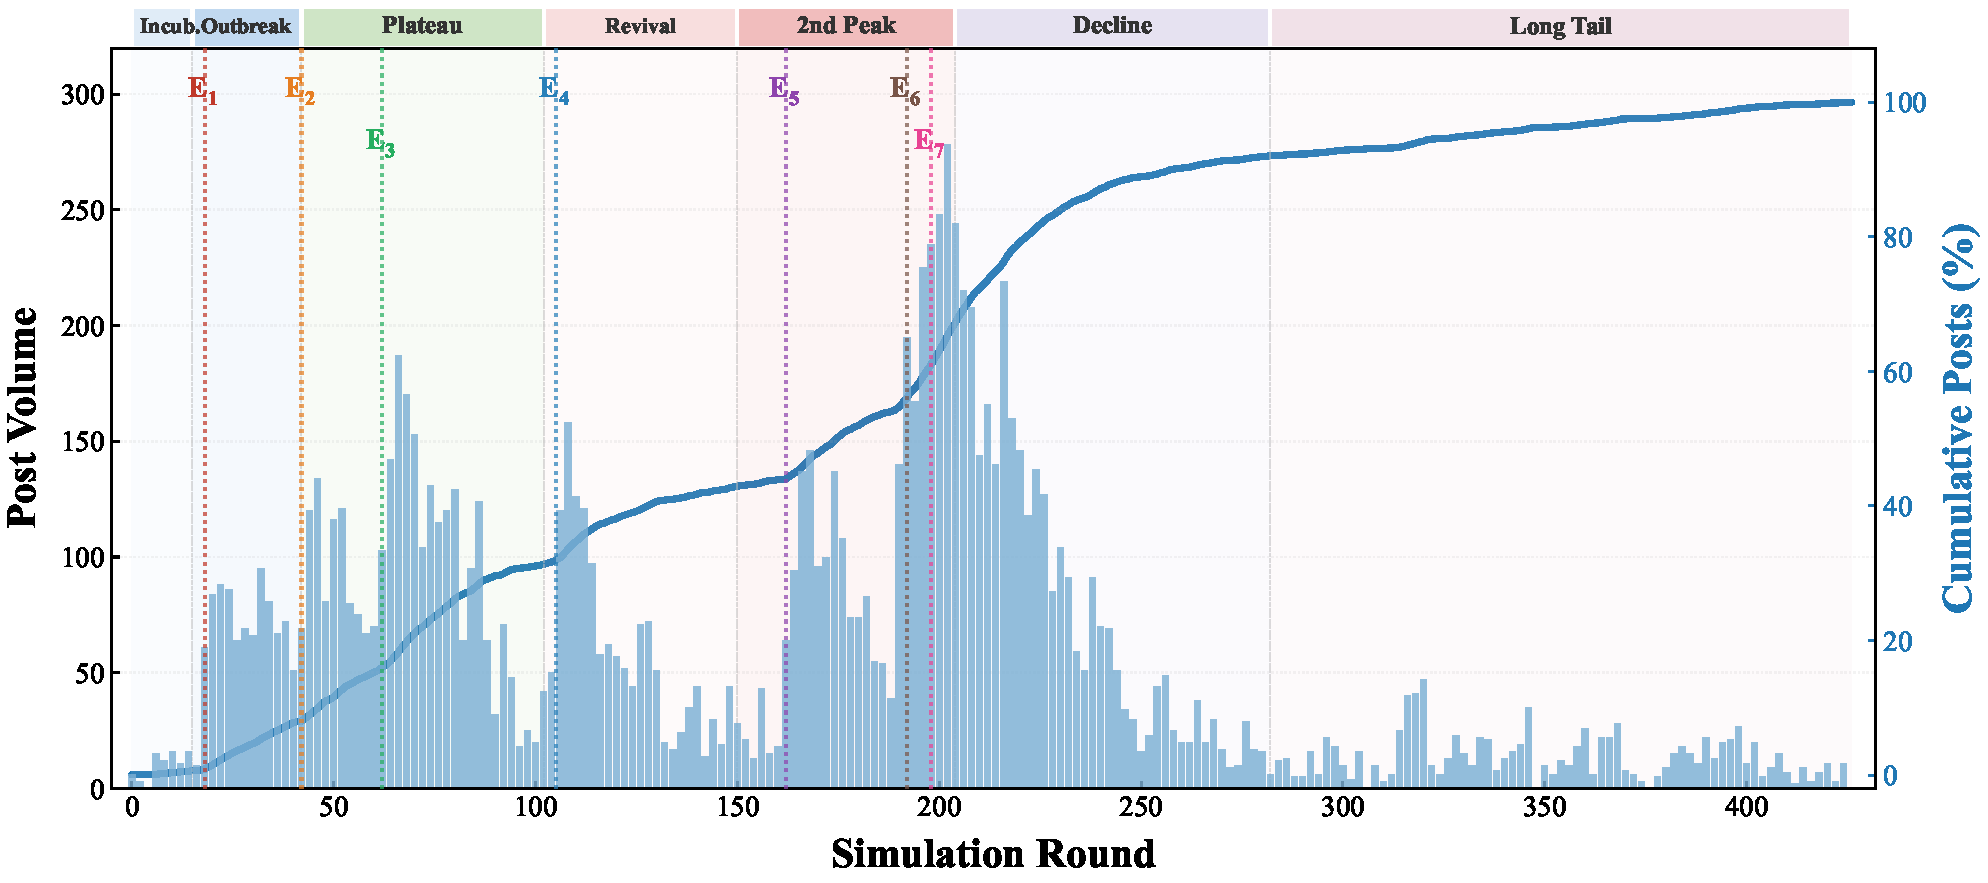
\includegraphics[width=0.82\textwidth]{fig_lifecycle_paper.pdf}
\caption{仿真舆情生命周期：发博量变化（柱状图，左轴）与累积发博百分比的观测S曲线（实线，右轴）及Logistic拟合曲线（虚线）。$E_1$--$E_7$标记外生事件注入时间点。}
\label{fig:lifecycle}
\end{figure*}

如图~\ref{fig:lifecycle}所示，仿真清晰展现了舆情从爆发、平台、复燃到衰退的多阶段生命周期，且各阶段转换均可溯源至特定事件的因果驱动。$E_1$（食品卫生视频曝光）注入后发博量迅速攀升，$E_2$（罗永浩宣布停战）后活跃度明显回落；$E_4$（创始人群聊截图流出）重新点燃停战默契，$E_5$（三大央媒同日发声）触发全程最大活跃度，呈现典型的死灰复燃和央媒定调引发二次爆发的效应。从累积发博的S型曲线来看，实际观测值在平台期持续低于Logistic拟合、在复燃期显著高于拟合，呈阶梯式S型偏离，拐点与$E_5$高度吻合。

\subsubsection{多主体行为异质性}

% --- 异质性图（双栏） ---
\begin{figure*}[!t]
\centering

\includegraphics[width=\textwidth]{fig_paper_heterogeneity.pdf}
\caption{四类智能体行为异质性：(a)~情绪强度时序演化；(b)~内容长度分布；(c)~多维行为特征雷达图。}
\label{fig:heterogeneity}
\end{figure*}

图~\ref{fig:heterogeneity}从情绪强度、内容长度和多维行为画像三个角度展示了四类智能体涌现出的系统性异质性。Citizen和KOL的平均情绪强度分别为0.645和0.603，始终处于高区间；Media和Government则稳定在低唤醒区间，分别为0.266和0.128，呈现公众情绪化、官方中性化的分层模式。内容长度呈阶梯分布：Media最长，均值为100.2字；Government次之，为90.6字；KOL为73.3字；Citizen最短，仅43.4字。雷达图上四类智能体形成了形态截然不同的多边形——Citizen偏向情绪多样性和活跃度，KOL最为均衡，Media和Government集中在影响力、内容深度和原创比例上——直观证明了EBDI架构成功将差异化的角色设定转化为可辨识的宏观行为异质性。

\subsubsection{情绪唤醒与极化效应}

基于情绪唤醒理论和情绪传染假说，我们从唤醒自增强和情绪传染两个维度进行验证（表~\ref{tab:emotion}）。

\begin{table}[!t]
\centering
\caption{情绪唤醒理论验证指标}
\label{tab:emotion}
\renewcommand{\arraystretch}{1.0}
\resizebox{\columnwidth}{!}{%
\begin{tabular}{@{}llcc@{}}
\toprule
\textbf{维度} & \textbf{指标} & \textbf{仿真结果} & \textbf{理论预期} \\
\midrule
\multirow{3}{*}{\makecell[l]{唤醒\\自增强}}
 & 高唤醒趋势系数 $\beta$ & $3.41{\times}10^{-4}$\,($p{<}0.001$) & $\beta > 0$ \\
 & 高唤醒情绪占比 & 73.5\% & 占主导 \\
 & 高/低唤醒强度比 & 2.0$\times$ & $>1$ \\
\midrule
\multirow{2}{*}{\makecell[l]{情绪\\传染}}
 & 评论链情绪一致率 & 0.772 & $\gg$ 随机基线 \\
 & 升级/降级比 & 4.78 & $>1$ (棘轮效应) \\
\bottomrule
\end{tabular}%
}
\end{table}

高唤醒情绪占比随仿真推进呈显著上升趋势，趋势系数$\beta = 3.41{\times}10^{-4}$且$p < 0.001$，总占比达73.5\%。高唤醒行为的平均情绪强度为0.658，显著高于低唤醒行为的0.328，差异倍率达$2.0\times$，与Berger和Milkman所预测的正反馈机制一致：高唤醒内容因传播优势获得更多曝光，进而激发更多高唤醒反应。在情绪传染方面，评论链中子评论与父帖的情绪一致率高达0.772，远超随机基线。升级/降级比为4.78，即由低唤醒转向高唤醒的概率是由高转低的近5倍，形成显著的棘轮效应，推动群体情绪不可逆地螺旋升级，支持Hatfield等人的情绪传染假说。

与此同时，我们定义极化指数$\text{PI} = 1 - H/H_{\max}$，其中$H$为各轮次的情绪Shannon熵，$H_{\max} = \log_2 K$（$K$为情绪类别数）。PI越高表示情绪分布越集中于少数类别。

\begin{figure}[!t]
\centering

\includegraphics[width=0.85\columnwidth]{fig_paper_polarization.pdf}
\caption{情绪极化指数（PI）随仿真轮次的演化。实线为PI均值，阴影为90\% Bootstrap置信区间，虚线标注早期与晚期均值。}
\label{fig:polarization}
\end{figure}

如图~\ref{fig:polarization}所示，极化指数从早期的0.41攀升至晚期的0.67（升幅63\%，$p < 0.001$），群体情绪从多元共存逐渐收敛为以少数高唤醒情绪主导的集中格局。该趋势与回音室理论一致：在信息推荐和社交互动的双重作用下，智能体逐渐被同质化的高唤醒情绪信息包围，情绪多样性不可逆地衰减。情绪极化与唤醒自增强共同构成了高唤醒驱动传播优势、进而导致多样性丧失的涌现因果链。

\subsubsection{无标度拓扑与级联幂律}

% --- 幂律图（双栏） ---
\begin{figure*}[!t]
\centering

\includegraphics[width=0.75\textwidth]{fig_paper_powerlaw.pdf}
\caption{互动网络的拓扑特性：(a)~度分布幂律拟合$P(k) \sim k^{-\gamma}$；(b)~级联规模CCDF$P(X \geq s) \sim s^{-\alpha}$。}
\label{fig:powerlaw}
\end{figure*}

真实社交网络的度分布和信息级联规模普遍服从幂律分布，是无标度网络和长尾传播的标志性特征。我们构建了基于评论和转发关系的互动网络，检验仿真输出是否涌现出上述拓扑规律。

如图~\ref{fig:powerlaw}(a)所示，互动网络的度分布在双对数坐标下呈良好线性关系，幂律拟合指数$\gamma = 1.87$（$R^2 = 0.880$），表明网络具有无标度特性——少数节点获得了极高的度值（最大度75），而大多数节点度值较低。该幂律指数落在真实社交网络中普遍报告的$1.5 < \gamma < 3$范围内，且Top-20\%用户贡献了51.3\%的互动量，体现了帕累托分布特征。

如图~\ref{fig:powerlaw}(b)所示，信息级联规模的CCDF在双对数坐标下同样呈线性衰减，$\alpha = 3.70$（$R^2 = 0.880$），拟合优度良好。5,473个级联中，中位数规模仅为1但最大达11，呈典型长尾效应——绝大多数内容获得有限传播，而少数内容形成相对大规模的级联。级联幂律指数$\alpha > 2$与有限病毒式传播特征一致，验证了仿真在信息传播动力学层面的保真度。

\subsection{统计结果校准}

本节将仿真输出与三个真实舆情事件进行直接对比，从\textbf{行为层}（行为类型分布与活跃度曲线）、\textbf{内容层}（话语对抗性、词汇多样性与情感倾向）和\textbf{拓扑层}（网络结构与信息级联）三个维度进行系统性校准。

\subsubsection{评估指标}

为系统量化仿真与真实数据的一致性，我们设计了覆盖三个层面的评估指标体系。

\textbf{行为层}包含三个指标：（1）行为类型分布散度（BType JSD），采用Jensen-Shannon散度度量模拟与真实行为类型（原创、转发、评论）概率分布的差异：
\begin{equation}
\text{JSD}(P \| Q) = \tfrac{1}{2} D_{\text{KL}}(P \| M) + \tfrac{1}{2} D_{\text{KL}}(Q \| M)
\end{equation}
其中$M = \frac{1}{2}(P + Q)$，JSD值越低表示越接近真实；（2）行为量曲线Pearson相关系数（Act.\,$\rho$），衡量模拟与真实的行为量时序曲线之间的趋势一致性；（3）行为量曲线RMSE（Act.\,RMSE），衡量归一化后行为量曲线的绝对偏差。

\textbf{内容层}包含三个指标：（1）话语对抗性相似度（Confr.\,Sim.），通过关键词检测评估对抗性表达比率的差异$\text{Confr.} = 1 - |c_{sim} - c_{real}|$；（2）词汇多样性偏差（$|\Delta\text{TTR}|$），计算Type-Token Ratio的绝对差异，TTR定义为唯一词元数与总词元数之比；（3）情感均值偏差（$|\Delta\bar{S}|$），计算模拟与真实内容情感极性均值的绝对差异。

\textbf{拓扑层}包含两个指标：（1）网络结构相似度（Net.\,Sim.），综合比较模拟与真实转发网络的入度分布、出度分布和网络密度等拓扑特征的加权相似度；（2）级联规模分布相似度（Casc.\,Sim.），将信息级联的规模分组为直方图，通过直方图交集度量分布一致性。各层平均得分（Avg.）对$\downarrow$指标取$1{-}x$后求均值。

\subsubsection{校准结果}

% --- 统计校准主表 ---
\begin{table*}[!t]
\centering
\caption{三个事件的统计校准结果（LE\,=\,天价耳环，WL\,=\,武大图书馆，XF\,=\,西贝预制菜）。\textbf{加粗}为各数据集最优；\na 表示不适用。}
\label{tab:calibration}
\vspace{2pt}
\renewcommand{\arraystretch}{1.18}
\resizebox{\textwidth}{!}{%
\footnotesize
\begin{tabular}{@{}cl cccc cccc ccc@{}}
\toprule
\multirow{2}{*}{\textbf{数据}} & \multirow{2}{*}{\textbf{方法}}
& \multicolumn{4}{c}{\textbf{行为层}}
& \multicolumn{4}{c}{\textbf{内容层}}
& \multicolumn{3}{c}{\textbf{拓扑层}} \\
\cmidrule(lr){3-6} \cmidrule(lr){7-10} \cmidrule(lr){11-13}
& & \makecell{行为类型\\JSD\,$\downarrow$} & \makecell{活跃度\\$\rho$\,$\uparrow$} & \makecell{活跃度\\RMSE\,$\downarrow$} & \makecell{均值\\$\uparrow$}
& \makecell{对抗性\\相似度\,$\uparrow$} & \makecell{$|\Delta\text{TTR}|$\\$\downarrow$} & \makecell{$|\Delta\bar{S}|$\\$\downarrow$} & \makecell{均值\\$\uparrow$}
& \makecell{网络\\相似度\,$\uparrow$} & \makecell{级联\\相似度\,$\uparrow$} & \makecell{均值\\$\uparrow$} \\
\midrule
\multirow{4}{*}{\textbf{LE}}
& Rule-based ABM        & 0.275 & 0.738 & 0.172 & 0.764 & \na & \na & \na & \na & 0.530 & 0.310 & 0.420 \\
& POSIM w/o EBDI        & 0.295 & 0.768 & 0.165 & 0.769 & 0.885 & 0.282 & 0.254 & 0.783 & 0.755 & 0.742 & 0.749 \\
& POSIM w/ CoT          & 0.225 & 0.785 & 0.161 & 0.800 & 0.882 & 0.145 & 0.105 & 0.877 & 0.768 & 0.785 & 0.777 \\
\rowcolor{oursrow}
& \textbf{POSIM (Ours)}  & \best{0.193} & \best{0.809} & \best{0.154} & \best{0.821} & \best{0.893} & \best{0.041} & \best{0.029} & \best{0.941} & \best{0.779} & \best{0.845} & \best{0.812} \\
\midrule
\multirow{4}{*}{\textbf{WL}}
& Rule-based ABM        & 0.255 & 0.713 & 0.120 & 0.779 & \na & \na & \na & \na & 0.547 & 0.285 & 0.416 \\
& POSIM w/o EBDI        & 0.322 & 0.733 & 0.136 & 0.758 & 0.888 & 0.311 & 0.342 & 0.745 & \best{0.837} & 0.729 & \best{0.783} \\
& POSIM w/ CoT          & 0.155 & 0.742 & 0.126 & 0.820 & 0.942 & 0.180 & 0.252 & 0.837 & 0.792 & 0.748 & 0.770 \\
\rowcolor{oursrow}
& \textbf{POSIM (Ours)}  & \best{0.073} & \best{0.750} & \best{0.118} & \best{0.853} & \best{0.985} & \best{0.011} & \best{0.203} & \best{0.924} & 0.772 & \best{0.761} & 0.767 \\
\midrule
\multirow{4}{*}{\textbf{XF}}
& Rule-based ABM        & 0.295 & 0.719 & 0.171 & 0.751 & \na & \na & \na & \na & 0.637 & 0.325 & 0.481 \\
& POSIM w/o EBDI        & 0.413 & 0.708 & 0.178 & 0.706 & \best{0.996} & 0.411 & \best{0.019} & 0.855 & 0.782 & \best{0.715} & \best{0.749} \\
& POSIM w/ CoT          & 0.215 & 0.718 & 0.173 & 0.777 & 0.950 & 0.198 & 0.038 & 0.905 & 0.784 & 0.702 & 0.743 \\
\rowcolor{oursrow}
& \textbf{POSIM (Ours)}  & \best{0.148} & \best{0.727} & \best{0.168} & \best{0.804} & 0.972 & \best{0.020} & 0.046 & \best{0.969} & \best{0.789} & 0.707 & 0.748 \\
\bottomrule
\end{tabular}%
}
\vspace{2pt}
{\scriptsize \textit{注：}Rule-based ABM依赖模板生成，无定向交互，内容层和级联指标不适用。均值对$\downarrow$指标取$1{-}x$后求平均。}
\end{table*}

实验在三个真实舆情数据集上开展，结果如表~\ref{tab:calibration}和图~\ref{fig:three_event_calibration}所示。

\begin{figure*}[!t]
\centering

\includegraphics[width=0.88\textwidth]{fig_three_event_calibration.pdf}
\caption{三个事件的统计校准可视化。每行对应一个事件（(a)~天价耳环、(b)~武大图书馆、(c)~西贝预制菜），左侧为模拟与真实数据的活跃度时序对比，右侧为行为类型的比例分布对比。}
\label{fig:three_event_calibration}
\end{figure*}

\textbf{行为层校准。}行为层校准从行为类型分布和行为量时序曲线两个角度评估仿真与真实数据的一致性。POSIM在三个数据集上的BType JSD均取得最优（LE: 0.193, WL: 0.073, XF: 0.148），说明EBDI元认知架构产生的行为决策在类型比例上与真实数据高度一致。值得注意的是，移除EBDI架构后（w/o EBDI），行为分布偏差显著增大，尤其在XF数据集上JSD从0.148升至0.413，表明分层认知推理对行为决策的类型多样性起到了关键调控作用。在行为量曲线校准方面，POSIM在所有数据集上均获得最高的Pearson相关系数和最低的RMSE。w/~CoT方法虽然引入了思维链推理，但由于缺乏信念-欲望-意图的分层建模，其行为层整体拟合精度仍低于完整的POSIM框架。行为层平均得分在三个数据集上分别达到0.821、0.853和0.804，均为所有方法中最高。

\textbf{内容层校准。}内容层校准评估仿真生成内容与真实内容在话语对抗性、词汇多样性和情感倾向上的相似性。传统的Rule-based ABM由于仅使用模板化文本输出，内容层指标不适用，这恰恰凸显了LLM驱动的仿真方法在内容生成层面的本质优势。在LLM驱动方法的对比中，POSIM的词汇多样性差异$|\Delta\text{TTR}|$在所有数据集上均最小（LE: 0.041, WL: 0.011），表明EBDI架构通过分层认知推理有效避免了平均人格问题，使得不同智能体产生差异化的文本输出。相比之下，w/o EBDI方法的TTR偏差显著偏大，说明缺乏结构化认知建模时智能体的文本输出趋于同质化。在情感校准方面，POSIM在LE数据集上实现了仅0.029的情感均值偏差。XF数据集上w/o EBDI方法的情感偏差虽更小（0.019 vs 0.046），但其在行为和词汇维度的系统性劣势表明这种局部一致性并非来自对真实认知过程的有效建模。内容层平均得分在三个数据集上分别为0.941、0.924和0.969，全面优于其他方法。

\textbf{拓扑层校准。}拓扑层校准从网络结构和信息级联两个角度评估仿真与真实社交网络的结构相似性。Rule-based ABM由于未建模用户间的定向交互关系，网络结构和级联规模相似度均明显偏低（拓扑层平均仅0.42--0.48），反映了传统规则驱动方法在建模社交互动结构方面的根本性缺陷。在LLM驱动方法中，POSIM在LE上取得最优的拓扑层指标（级联规模相似度达0.845）。在WL和XF上，w/o EBDI方法的拓扑层平均略高（分别为0.783 vs 0.767和0.749 vs 0.748），这是因为拓扑结构主要受环境层的推荐机制和霍克斯点过程驱动，与认知架构的直接关联较弱。然而，从全局视角来看，POSIM在行为和内容两个与认知决策直接相关的层面上具有显著且一致的优势。

\textbf{综合分析。}综合三个层面的校准结果，POSIM在行为层和内容层全面领先，在拓扑层保持高度竞争力。这得益于EBDI架构的三方面贡献：（1）分层信念更新机制使智能体能够根据不同类型信息的可信度进行差异化的认知修正，从而产生更符合真实人类特征的行为分布；（2）基于欲望驱动的动机生成避免了直接提示方式的理性人偏差，使不同心理特征的智能体展现出差异化的行为倾向；（3）多级意图规划保证了内容生成的策略多样性，有效提升了词汇丰富度和话语风格的异质性。

\subsection{消融实验}

为验证POSIM各核心模块的必要性，我们以天价耳环事件（LE）为基准，设置完整框架（Full POSIM）与若干变体配置进行对比，结果如表~\ref{tab:ablation}所示。

\begin{table}[!t]
\centering
\caption{消融实验结果（LE数据集）}
\label{tab:ablation}
\renewcommand{\arraystretch}{1.0}
\resizebox{\columnwidth}{!}{%
\begin{tabular}{@{}l ccc ccc cc@{}}
\toprule
\multirow{2}{*}{\textbf{配置}} & \multicolumn{3}{c}{\textbf{行为层}} & \multicolumn{3}{c}{\textbf{内容层}} & \multicolumn{2}{c}{\textbf{拓扑层}} \\
\cmidrule(lr){2-4} \cmidrule(lr){5-7} \cmidrule(lr){8-9}
& \makecell{JSD\\$\downarrow$} & \makecell{$\rho$\\$\uparrow$} & \makecell{RMSE\\$\downarrow$}
& \makecell{对抗性\\$\uparrow$} & \makecell{$|\Delta$TTR$|$\\$\downarrow$} & \makecell{$|\Delta\bar{S}|$\\$\downarrow$}
& \makecell{网络\\$\uparrow$} & \makecell{级联\\$\uparrow$} \\
\midrule
\rowcolor{greenrow}
Full POSIM & \best{0.193} & \best{0.809} & \best{0.154} & \best{0.893} & \best{0.041} & \best{0.029} & \best{0.779} & \best{0.845} \\
w/o Belief & --- & --- & --- & --- & --- & --- & --- & --- \\
\rowcolor{grayrow}
w/o Desire & --- & --- & --- & --- & --- & --- & --- & --- \\
w/o Hawkes & --- & --- & --- & --- & --- & --- & --- & --- \\
\bottomrule
\end{tabular}%
}
\end{table}

（本节暂不展开各模块的独立贡献分析，未来版本将补充系统性的消融实验与结果解读。）


% ============================================================
% 第5节 案例研究（占位，后续步骤填充）
% ============================================================
\section{案例研究}
\label{sec:case}

前述验证实验证明了POSIM在再现真实舆情方面的有效性。本节进一步展示POSIM作为计算实验平台的应用价值——通过认知引导实验和反事实策略干预实验，演示框架在因果推理和策略评估方面的能力。

\subsection{认知引导实验}

认知引导实验旨在回答：如果在舆情爆发前改变用户的认知信念，群体层面的舆情动态会如何变化？实验设计4种条件：\textbf{对照组}（不修改信念）、\textbf{理性认知引导}（RC，预设理性思维和中立观点）、\textbf{共情引导}（EP，预设换位思考和尊重性信念）和\textbf{情绪调节}（ER，重置情绪向量并预设情绪管理信念），均在100\%覆盖率下实施。实验选取200个智能体模拟天价耳环事件爆发后5小时（30步），评估负面情绪比例（NER）、愤怒比例、情绪强度和正面情绪比例。结果见表~\ref{tab:priming}。

\begin{table}[!t]
\centering
\caption{认知引导实验结果（100\%覆盖率，200智能体，30步）}
\label{tab:priming}
\renewcommand{\arraystretch}{1.0}
\small
\begin{tabular}{@{}lcccc@{}}
\toprule
\textbf{条件} & \makecell{\textbf{负面情绪}\\\textbf{比例}\,$\downarrow$} & \makecell{\textbf{愤怒}\\\textbf{比例}\,$\downarrow$} & \makecell{\textbf{情绪}\\\textbf{强度}\,$\downarrow$} & \makecell{\textbf{正面}\\\textbf{情绪}\,$\uparrow$} \\
\midrule
对照组 & 0.844 & 0.600 & 0.649 & 0.010 \\
\rowcolor{orangerow}
理性认知引导 (RC) & \best{0.571} & \best{0.407} & \best{0.527} & 0.017 \\
\rowcolor{grayrow}
共情引导 (EP) & 0.878 & 0.569 & 0.650 & 0.005 \\
情绪调节 (ER) & 0.572 & 0.481 & 0.573 & \best{0.066} \\
\bottomrule
\end{tabular}
\end{table}

% --- 认知引导图占位 ---
\begin{figure}[!t]
\centering

\includegraphics[width=\columnwidth]{paper_cognitive_priming.pdf}
\caption{认知引导实验：(a)~100\%覆盖率下四种条件的NER时序演化；(b)~三种策略的NER变化幅度随覆盖率的剂量-效应关系。}
\label{fig:priming}
\end{figure}

实验揭示了四个关键发现。\textbf{（1）RC和ER策略显著降低负面情绪，且呈现剂量效应。}如图~\ref{fig:priming}所示，RC将负面情绪比例从0.844降至0.571（降幅32.3\%），整体情绪强度也明显下降。图~\ref{fig:priming}(b)显示RC的覆盖率跨越60\%后效果显著跃升，呈现阈值效应。\textbf{（2）共情悖论效应。}EP的负面情绪比例为0.878，反而高于对照组的0.844，且随覆盖率增大反而上升，呈现反剂量效应。这一悖论在社会心理学中已有理论预期——共情理解他人痛苦的同时会产生更多移情性负面情绪——在仿真中首次被定量观察到。\textbf{（3）ER策略在正面情绪提升上独具优势。}ER的正面情绪比例达0.066，远高于RC的0.017，揭示了感受层调控与认知层引导的机制差异。\textbf{（4）行为总量保持稳定。}各条件下的行为总量高度一致，变异系数仅4.6\%，表明EBDI架构实现了行为动机与情绪表达的有效解耦。

\subsection{反事实策略评估}

基于西贝预制菜事件设计反事实实验，保持外部事件不变，仅替换西贝的公关响应，比较五种策略：\textbf{实际应对}（AR，从强硬否认、自曝到辱骂、秒删致歉）、\textbf{及时致歉}（SEA）、\textbf{主动透明}（PT）、\textbf{消费者对话}（CD）和\textbf{战略沉默}（SS）。每种策略使用200个智能体、20步仿真，策略在第4步和第12步部署。结果见表~\ref{tab:counter}。

\begin{table}[!t]
\centering
\caption{反事实策略评估结果（200智能体，20步）}
\label{tab:counter}
\renewcommand{\arraystretch}{1.0}
\small
\begin{tabular}{@{}lcccc@{}}
\toprule
\textbf{策略} & \makecell{\textbf{负面情绪}\\\textbf{比例}\,$\downarrow$} & \makecell{\textbf{愤怒}\\\textbf{比例}\,$\downarrow$} & \makecell{\textbf{情绪}\\\textbf{强度}\,$\downarrow$} & \makecell{\textbf{正面}\\\textbf{情绪}\,$\uparrow$} \\
\midrule
实际应对 (AR) & 0.792 & 0.791 & 0.685 & 0.000 \\
\rowcolor{grayrow}
及时致歉 (SEA) & 0.749 & 0.749 & 0.612 & 0.002 \\
主动透明 (PT) & 0.773 & 0.773 & 0.645 & 0.002 \\
\rowcolor{purplerow}
消费者对话 (CD) & \best{0.744} & \best{0.743} & \best{0.598} & \best{0.005} \\
\rowcolor{grayrow}
战略沉默 (SS) & 0.831 & 0.831 & 0.702 & 0.004 \\
\bottomrule
\end{tabular}
\end{table}

% --- 反事实策略图（双栏） ---
\begin{figure*}[!t]
\centering
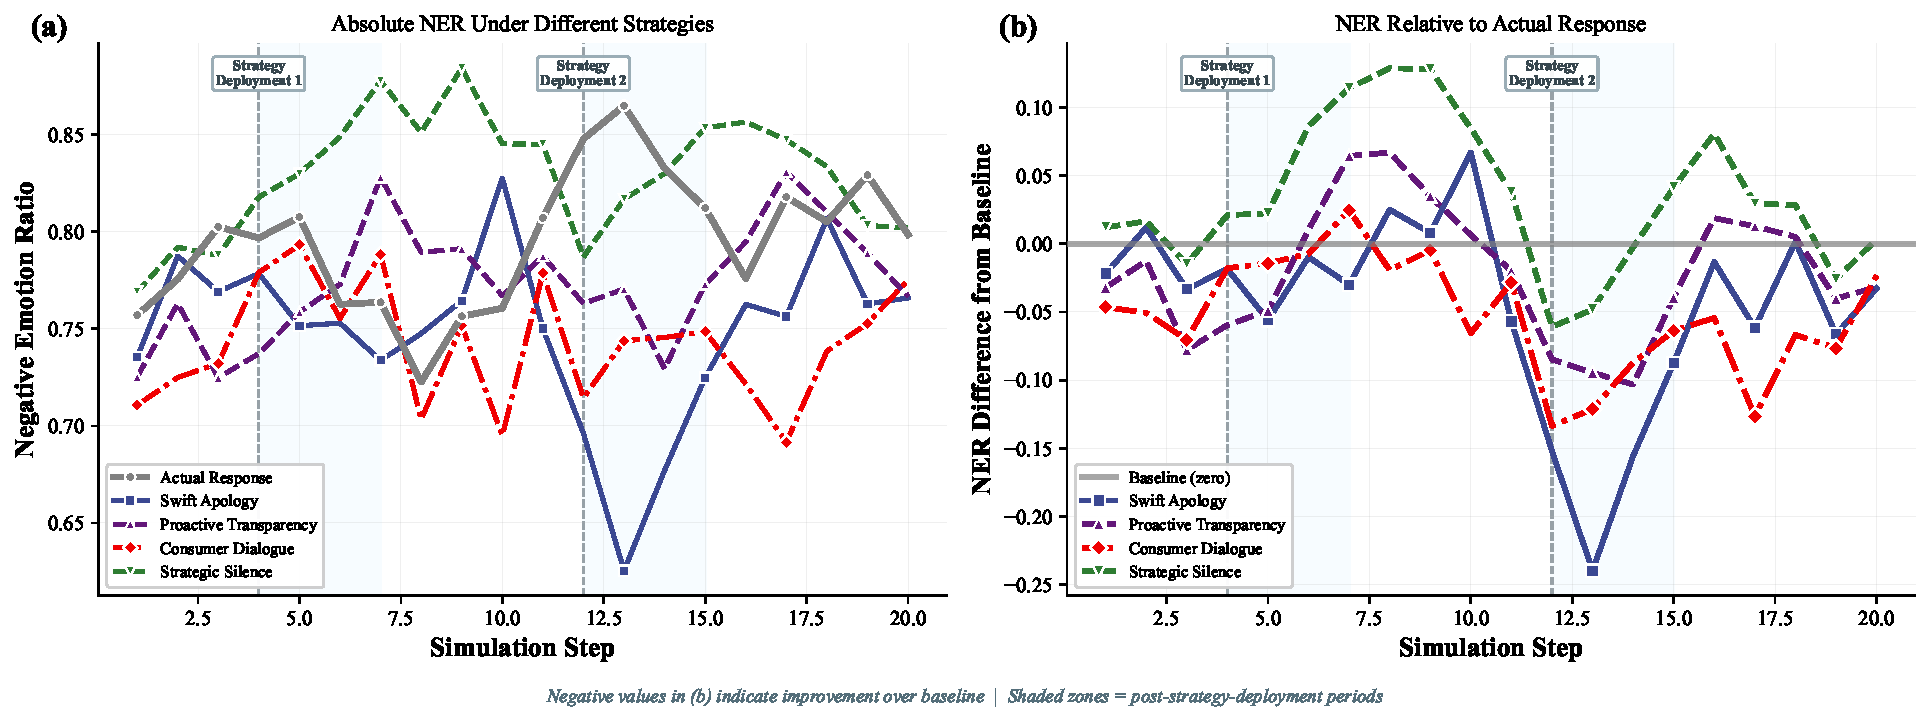
\includegraphics[width=0.82\textwidth]{paper_strategy_comparison.pdf}
\caption{反事实策略评估：(a)~五种公关策略下NER的时序演化（滚动平均），蓝色阴影标记策略部署时间点；(b)~各策略相对于实际应对基线的NER差值。}
\label{fig:counterfactual}
\end{figure*}

实验揭示了三个关键发现。\textbf{（1）积极策略显著优于消极应对，CD策略效果最优。}SEA次之，NER为0.749；PT第三，为0.773。\textbf{（2）战略沉默表现最差。}沉默策略仅对30\%的智能体产生轻微信念修正，绝大多数智能体的事件观点信念维持原始负面状态，验证了危机公关中沉默并非最优选择的教训。\textbf{（3）策略效果呈即时降温与逐步反弹的动态模式。}时序分析显示，SEA在部署后NER一度降至0.56，但随后在负面内容推荐的持续作用下逐步回升，精确模拟了真实舆情中公关效果衰减的常见现象。策略传导严格遵循信念修正、认知推理改变、行为输出转变的因果链条，验证了EBDI架构在策略评估中的可解释性优势。


% ============================================================
% 第6节 结论（占位，后续步骤填充）
% ============================================================
\section{结论}
\label{sec:conclusion}

本文提出了社交媒体舆情仿真框架POSIM，通过将大语言模型嵌入EBDI分层认知架构构建元认知智能体，结合霍克斯自激点过程驱动的仿真环境，实现了高保真的舆情演化仿真。

\textbf{主要发现。}通过三个层次的系统验证，我们得出以下关键结论：（1）EBDI元认知架构在微观层面显著优于直接提示和思维链方法，在认知行为链一致性、人格稳定性和认知鲁棒性上均全面领先，支持多步独立认知架构在微观行为机制校准上的有效性；（2）仿真系统能够自发涌现出与社会科学理论一致的宏观现象，包括事件驱动的多阶段生命周期、四类智能体的系统性行为异质性、情绪唤醒自增强与极化效应、以及无标度网络拓扑和级联幂律分布；（3）在统计校准层面，POSIM在三个数据集上的行为层和内容层平均得分全面优于基线方法，验证了框架在统计层面的高保真度。

\textbf{应用价值。}案例研究展示了POSIM作为计算实验平台的独特应用价值。认知引导实验中，共情悖论效应——共情引导反而增加负面情绪——在仿真中首次被定量观察到，证明LLM认知智能体能捕捉到认知科学中更细微的非线性效应，而非仅简单再现引导即改善的线性因果链。反事实策略评估实验中，五种公关策略的量化对比为危机公关策略的优选提供了实证依据，其中消费者对话策略最优、战略沉默最差的结论与公关理论预期一致但首次获得仿真层面的定量支撑。策略效果呈现的即时降温与逐步反弹的动态模式，揭示了信念修正的时效性特征，为现实中的舆情治理提供了策略持续性方面的决策参考。

\textbf{局限与展望。}本研究存在以下局限：（1）框架的认知推理质量受限于底层LLM的能力，不同模型可能产生不同的仿真结果，且大规模仿真的API成本仍有优化空间；（2）当前实现中用户间的关注关系在仿真过程中保持静态，未建模关注/取消关注的动态演化；（3）实验仅在微博平台数据上验证，跨平台（如微信、抖音）的迁移能力有待检验；（4）部分微观指标依赖LLM-as-Judge评估，可能存在评估偏差。未来工作将探索动态社交网络建模、多平台适配、更高效的LLM调用策略以及更丰富的干预机制设计。


% ============================================================
% 参考文献
% ============================================================
\bibliographystyle{IEEEtran}
\bibliography{posim_refs}


% ============================================================
% 附录（占位，后续步骤填充）
% ============================================================

\appendices

% ============================================================
% 附录A：核心算法伪代码
% ============================================================
\section{核心算法伪代码}

\begin{algorithm}[!t]
\caption{POSIM仿真主循环}
\label{alg:main}
\begin{algorithmic}[1]
\REQUIRE 智能体集合$\mathcal{U}$，事件队列$\mathcal{E}$，配置$\mathcal{C}$
\ENSURE 仿真轨迹$\mathcal{T}$
\STATE 初始化霍克斯过程$\mathcal{H}(\mu, \alpha_{int}, \beta_{int}, \alpha_{ext}, \beta_{ext})$
\STATE 初始化推荐系统$\mathcal{R}$和热搜系统$\mathcal{S}$
\FOR{$t = 0, 1, \ldots, T_{max}$}
 \STATE $t_{sim} \leftarrow t_0 + t \cdot \Delta t$
 \STATE $\mathcal{E}_{cur} \leftarrow \mathcal{E}.\text{get\_events}(t_{sim})$
 \FORALL{$e \in \mathcal{E}_{cur}$}
 \STATE $\mathcal{H}.\text{add\_external}(t, e.\text{influence})$
 \ENDFOR
 \STATE 计算$\lambda_{adj}(t)$（式\ref{eq:hawkes}--\ref{eq:circadian}）
 \STATE $N_t \leftarrow \text{Poisson}(\lambda_{adj}(t) \cdot N_{scale} \cdot \Delta t / 60)$
 \STATE $\mathcal{A}_t \leftarrow \text{WeightedSample}(\mathcal{U}, N_t)$
 \FORALL{$u \in \mathcal{A}_t$ \textbf{parallel}}
 \STATE $P_t \leftarrow \mathcal{R}.\text{recommend}(u, t_{sim})$
 \STATE $I_u \leftarrow \text{EBDI-Pipeline}(u, P_t, \mathcal{E}_{ctx})$ \COMMENT{算法\ref{alg:ebdi}}
 \STATE 执行$I_u$并更新$\mathcal{H}$
 \ENDFOR
 \STATE 执行情绪传染；更新热搜榜$\mathcal{S}$
 \STATE $\mathcal{T} \leftarrow \mathcal{T} \cup \{(t, \mathcal{A}_t, I)\}$
\ENDFOR
\RETURN $\mathcal{T}$
\end{algorithmic}
\end{algorithm}

\begin{algorithm}[!t]
\caption{EBDI认知决策管线}
\label{alg:ebdi}
\begin{algorithmic}[1]
\REQUIRE 智能体$u$，环境感知$P_t$，事件上下文$\mathcal{E}_{ctx}$
\ENSURE 行为序列$I_t$
\STATE \textbf{阶段1：信念更新}
\STATE $M_t \leftarrow \text{StreamMemory.retrieve}(P_t, k)$
\STATE $B_t \leftarrow f_{\text{LLM}}(B_{t-1}, P_t, M_t, \Phi_{bias})$ \COMMENT{式\ref{eq:belief_update}}
\STATE $B_t.\text{emo} \leftarrow B_t.\text{emo} \odot e^{-\lambda_e \Delta t}$
\STATE \textbf{阶段2：欲望生成}
\STATE $D_t \leftarrow g_{\text{LLM}}(B_t, P_t)$
\STATE \textbf{阶段3：意图规划}
\STATE $L_1 \leftarrow \text{SelectActionType}(B_t, D_t, P_t)$
\STATE $L_2 \leftarrow \text{PlanStrategy}(L_1, B_t)$
\STATE $L_3 \leftarrow \text{GenerateContent}(L_1, L_2, B_t)$
\STATE $I_t \leftarrow h_{\text{LLM}}(B_t, D_t, P_t, L_1, L_2)$
\STATE \textbf{阶段4：记忆更新}
\STATE $\text{StreamMemory.store}(I_t, t)$
\RETURN $I_t$
\end{algorithmic}
\end{algorithm}

% ============================================================
% 附录B：核心提示词模板
% ============================================================
\section{核心提示词模板}
\label{app:prompts}

本附录展示普通网民智能体在EBDI认知架构中使用的三个核心提示词模板。

\begin{figure*}[!t]
\centering
\begin{minipage}[t]{0.48\textwidth}
\begin{promptbox}
\scriptsize
\textbf{B.1~~信念更新提示词 (Belief Update Prompt)}\\[3pt]
You are currently an ordinary netizen on the Weibo platform, participating in a public opinion event discussion.\\[2pt]
Current event background: \texttt{\{event\_background\}}\\[2pt]
\textbf{\#\# Belief State Inference}\\
Current time: \texttt{\{current\_time\}}\\[2pt]
Based on the following information, infer your current belief state:\\
\textbf{\#\#\# My Identity Information:} \texttt{\{identity\_text\}}\\
\textbf{\#\#\# My Previous Belief State:} \texttt{\{belief\_text\}}\\
\textbf{\#\#\# Newly Received Information:} \texttt{\{new\_info\}}\\
\textbf{\#\#\# My Historical Behavior Memory:} \texttt{\{memories\}}\\
\textbf{\#\#\# External Events:} \texttt{\{external\_events\}}\\[2pt]
Please consider the following cognitive bias mechanisms:\\
1. \textbf{Confirmation bias}: More likely to accept information consistent with existing views\\
2. \textbf{Anchoring effect}: Initially formed opinions exert disproportionate influence\\
3. \textbf{Emotional contagion}: Emotions influenced by affective tone of observed content\\
4. \textbf{Herd mentality}: Tendency to conform when the majority holds a certain view\\
5. \textbf{Emotion-first reasoning}: Emotional reactions precede rational analysis\\
6. \textbf{Simplistic attribution}: Tendency to oversimplify complex issues\\[2pt]
Output your current belief state in JSON format:
\begin{verbatim}
{"psychological_cognition": [...],
 "event_opinions": [{"subject": "...",
   "opinion": "...", "reason": "..."}],
 "emotion_vector": {"happiness": 0.0,
   "sadness": 0.0, "anger": 0.0,
   "fear": 0.0, "surprise": 0.0,
   "disgust": 0.0}}
\end{verbatim}
\vspace{-8pt}
\textit{Note: Each emotion dimension ranges in [0,1].}
\end{promptbox}
\end{minipage}
\hfill
\begin{minipage}[t]{0.48\textwidth}
\begin{promptbox}
\scriptsize
\textbf{B.2~~欲望生成提示词 (Desire Generation Prompt)}\\[3pt]
You are an ordinary netizen on the Weibo platform. Based on your current beliefs and information you have seen, infer your current social desires.\\[2pt]
Current event background: \texttt{\{event\_background\}}\\[2pt]
\textbf{\#\# Desire Reasoning}\\
Current time: \texttt{\{current\_time\}}\\[2pt]
As a Weibo platform user, based on my current beliefs and observed information, infer my current desires:\\
\textbf{\#\#\# My Current Belief State:} \texttt{\{belief\_text\}}\\
\textbf{\#\#\# Information I Have Seen:} \texttt{\{exposed\_info\}}\\
\textbf{\#\#\# External Events:} \texttt{\{external\_events\}}\\[2pt]
\textbf{Desire Types} (prioritized for ordinary netizens):\\
$\bullet$ \textit{Emotional venting}: Stress relief, expressing dissatisfaction\\
$\bullet$ \textit{Entertainment}: Watching the drama unfold, spectator mentality\\
$\bullet$ \textit{Self-expression}: Sharing opinions, displaying attitudes\\
$\bullet$ \textit{Social approval}: Seeking likes, followers, recognition\\
$\bullet$ \textit{Social connection}: Interacting with others\\
$\bullet$ \textit{Justice advocacy}: Upholding justice, defending rights\\
$\bullet$ \textit{Information seeking}: Understanding the truth\\[2pt]
Output the desire list in JSON format:
\begin{verbatim}
{"desire_list": [
  {"type": "emotional_venting",
   "description": "...",
   "intensity": "very_low | low |
                 medium | high |
                 very_high"},
  {"type": "information_seeking",
   "description": "...",
   "intensity": "..."}]}
\end{verbatim}
\end{promptbox}
\end{minipage}
\end{figure*}

\begin{figure*}[!t]
\centering
\begin{minipage}[t]{0.48\textwidth}
\begin{promptbox}
\scriptsize
\textbf{B.3~~意图与行为决策提示词 (Intention \& Action Prompt)}\\[3pt]
You are an ordinary netizen on the Weibo. Combine your beliefs, desires, and breaking events to decide actions.\\[2pt]
Background: \texttt{\{event\_background\}}\\[2pt]
\textbf{[Behavioral Characteristics]}\\
Language: colloquial, emotional, internet slang. Expression: exaggerated, biased allowed. Emotions expressed directly. Rapid response to breaking events.\\[2pt]
\textbf{[Decision Guidelines]}\\
Determine actions based on: event heat, emotional intensity, relevance, temporal decay, exposure content.\\[2pt]
\textbf{Three-level chain-of-thought reasoning:}\\[2pt]
\textbf{L1---Action type \& target:}\\
Choose among \textit{Like}, \textit{Repost}, \textit{Repost with comment}, \textit{Comment}, \textit{Original post}; specify the target post index for interactive behaviors.\\[2pt]
\textbf{L2---Expression strategy} (skip for Like/Repost without text):\\
$\bullet$ Emotion: type \& intensity\\
$\bullet$ Stance: support/oppose/neutral\\
$\bullet$ Style: sarcastic/aggressive/empathetic/\ldots\\
$\bullet$ Narrative: labeling/conspiracy/call-to-action/\ldots\\[2pt]
\textbf{L3---Content generation} (skip for pure Like):\\
Generate Weibo text matching netizen voice, consistent with L1 and L2.
\end{promptbox}
\end{minipage}
\hfill
\begin{minipage}[t]{0.48\textwidth}
\begin{promptbox}
\scriptsize
\textbf{B.3~~意图与行为决策提示词（续）}\\[3pt]
Output the full action list in JSON format:
\begin{verbatim}
{"action_list": [
  {"action_type": "comment",
   "target_id": "...",
   "expression_strategy": {
     "emotion": "...",
     "stance": "...",
     "style": "...",
     "narrative": "..."},
   "content": {"text": "..."}}]}
\end{verbatim}
\vspace{4pt}
\textbf{Important Notes:}\\[2pt]
$\bullet$ Action types include: \texttt{like}, \texttt{repost}, \texttt{repost\_with\_comment}, \texttt{comment}, \texttt{original\_post}\\[2pt]
$\bullet$ For \texttt{like} and pure \texttt{repost}, no content generation is needed\\[2pt]
$\bullet$ For \texttt{comment} and \texttt{repost\_with\_comment}, must specify \texttt{target\_id}\\[2pt]
$\bullet$ Expression strategy should align with current emotional state and desires\\[2pt]
$\bullet$ Content should reflect the persona characteristics defined in identity beliefs\\[2pt]
$\bullet$ Use internet slang and colloquial expressions appropriately for authenticity
\end{promptbox}
\end{minipage}
\end{figure*}
\section{参数配置}

\begin{table}[!t]
\centering
\caption{霍克斯点过程参数配置（三个事件统一）}
\label{tab:hawkes_params}
\renewcommand{\arraystretch}{1.0}
\resizebox{\columnwidth}{!}{%
\begin{tabular}{@{}llrl@{}}
\toprule
\textbf{参数} & \textbf{符号} & \textbf{取值} & \textbf{说明} \\
\midrule
背景活跃率 & $\mu$ & 0.01 & 无事件时的基础发博概率 \\
内生激励系数 & $\alpha_{int}$ & 0.005 & 用户行为的激励强度 \\
内生衰减率 & $\beta_{int}$ & 0.16 & 内生激励的衰减速率 \\
外生激励系数 & $\alpha_{ext}$ & 0.08 & 外部事件的激励强度 \\
外生衰减率 & $\beta_{ext}$ & 0.005 & 外生激励的衰减速率 \\
缩放因子 & $N_{scale}$ & 2000 & 强度到人数的缩放系数 \\
昼夜节律强度 & $s_{circ}$ & 0.3 & 昼夜节律调制权重 \\
\bottomrule
\end{tabular}%
}
\end{table}

\begin{table}[!t]
\centering
\caption{推荐系统参数配置}
\label{tab:rec_params}
\renewcommand{\arraystretch}{1.0}
\resizebox{\columnwidth}{!}{%
\begin{tabular}{@{}llrl@{}}
\toprule
\textbf{参数} & \textbf{符号} & \textbf{取值} & \textbf{说明} \\
\midrule
同质性权重 & $\alpha$ & 0.3 & 语义相似度权重 \\
热度权重 & $\beta$ & 0.3 & 互动热度权重 \\
新鲜度权重 & $\gamma$ & 0.2 & 时间衰减权重 \\
探索率 & $r_{explore}$ & 0.2 & 随机推荐比例 \\
推荐数量 & $K$ & 10 & 每步推荐博文数 \\
评论采样 & $N_c$ & 5 & 每条博文采样评论数 \\
嵌入模型 & --- & \multicolumn{2}{l}{BGE-small-zh-v1.5} \\
去重阈值 & $\theta_{dedup}$ & 0.92 & 语义去重余弦阈值 \\
\bottomrule
\end{tabular}%
}
\end{table}

% ============================================================
% 附录D：数据采集与预处理
% ============================================================
\section{数据采集与预处理}
\label{app:data}

本研究使用的三个舆情事件数据均从新浪微博平台采集。对于每个事件，数据采集范围包括：（1）包含事件相关话题标签或关键词的原创博文及其完整的转发链和评论树；（2）所有参与用户的基本信息（用户名、性别、地区、认证类型、粉丝数、个人描述等）。

\textbf{数据预处理流程。}原始数据经历以下多阶段清洗：（a）基于博文ID去除重复条目；（b）过滤事件期间发帖少于2条的低活跃用户，确保每个智能体具有足够的行为样本用于信念初始化；（c）基于关键词黑名单移除广告和垃圾内容（如``券后价''``拼多多''``包邮''等商业推广词汇）；（d）过滤与事件主题无关的内容（如``超话签到''``创业板''等无关话题）；（e）内容质量过滤：原创博文最小长度20字、转发和评论最小长度10字；（f）时间戳统一标准化至分钟级精度。

\textbf{信念初始化细节。}智能体信念初始化是数据预处理中最关键的环节。对于角色身份信念，将用户的基础信息和历史内容摘要输入LLM，以第一人称自述形式生成。心理认知信念从预定义的心理特征池（涵盖自我实现型、猎奇探究型、减压宣泄型、仇官仇富型、跟风从众型、情绪卷入型、娱乐消遣型、信息分享型八类模式，每类约30条代表性条目）中个性化采样。事件观点信念通过LLM驱动的结构化深度访谈（如提问``对于涉事主体X，你的观点是什么？''）提取。初始情绪向量基于用户近期发布内容的情感分析结果初始化。整个初始化过程支持多API并发处理和增量检查点保存，确保大规模用户池的高效初始化和故障恢复。

% ============================================================
% 附录E：计算效率分析
% ============================================================
\section{计算效率分析}

\begin{table}[!t]
\centering
\caption{三个事件仿真的计算资源消耗}
\label{tab:efficiency}
\renewcommand{\arraystretch}{1.0}
\begin{tabular}{@{}lrrr@{}}
\toprule
\textbf{指标} & \textbf{LE} & \textbf{WL} & \textbf{XF} \\
\midrule
智能体数 & 1,530 & 1,843 & 1,987 \\
仿真步数 & 276 & 1,140 & 426 \\
模拟时长 & $\sim$46h & $\sim$190h & $\sim$71h \\
行为总量 & 29,146 & 46,140 & 12,261 \\
LLM调用次数 & 26,295 & 39,945 & 11,670 \\
Token总量 & 28.98M & 46.95M & 13.37M \\
实际运行时间 & $\sim$3.5h & $\sim$8.3h & $\sim$1.9h \\
\bottomrule
\end{tabular}
\end{table}

表~\ref{tab:efficiency}报告了三个事件仿真的计算资源消耗。所有实验使用Qwen2.5-14B-Instruct模型，30路并发连接。每次智能体激活触发3次LLM调用，三事件合计约7.8万次调用，错误率低于0.006\%。得益于并发执行，实际运行时间控制在1.9--8.3小时。按当前定价，单次仿真API成本约10--35元，使大规模社会仿真在经济上完全可行。

% ============================================================
% 附录F：评估模型配置
% ============================================================
\section{评估模型配置}

微观行为机制验证（第\ref{sec:exp}节）中所有基于LLM-as-Judge的评估均使用Qwen2.5-14B-Instruct模型，通过硅基流动API调用，temperature设为0.3以保证评分一致性。每次评估调用遵循结构化提示词格式，包含：（1）带有各维度评分标准的评估量规；（2）智能体的完整行为轨迹记录；（3）参考信息（如用于人格稳定性评估的初始身份设定）。评估模型与仿真决策模型使用相同的模型家族和API基础设施，但在评估过程中保持独立调用，以避免自我评价偏差。评估过程中每条样本独立评分，不在样本间共享评分上下文，确保评分的独立性和无偏性。


\end{document}
